% 
\documentclass[10pt]{article}
\usepackage{amscd,amsfonts,amssymb,amstext,latexsym} 
\usepackage{amsmath,mathbbol,mathrsfs,stmaryrd, mathtools} 
%\usepackage{mathbbol,mathrsfs,stmaryrd}
\usepackage[ruled]{algorithm2e}
\usepackage{theoremref}
\usepackage[T1]{fontenc}
\usepackage[english]{babel} 
\usepackage {enumerate}
\usepackage{url}
%\usepackage {algpseudocode}  
\usepackage{graphics} 
\usepackage{tikz}
\usepackage[square]{natbib}
\usepackage[]{geometry}
\usetikzlibrary{automata,calc}
%\usepackage{tgtermes} 
\usepackage{listings}
\usepackage{mathptmx}
\usepackage{fancyhdr}
\usepackage{verbatim}
\usepackage{enumitem}
\usepackage{booktabs}
\usepackage[flushleft]{threeparttable}
\usepackage{listings}
\usepackage{verbatim}
\usepackage{fancyhdr}
\usepackage{multirow,multicol}
\usepackage[colorlinks=true,linkcolor=blue,citecolor=blue,urlcolor=blue]{hyperref}
\usepackage{tabto}
\lstset{ %
language=C++,                % choose the language of the code
basicstyle={\ttfamily},       % the size of the fonts that are used for the code
backgroundcolor=\color{white},  % choose the background color. You must add \usepackage{color}
showspaces=false,               % show spaces adding particular underscores
aboveskip=6mm, 
%belowskip=3mm, 
numbers=left, numberfirstline=false, numberblanklines=false,
numberstyle=\tiny\color{gray}, numbersep= 5pt, 
showstringspaces=false,         % underline spaces within strings
showtabs=false,                 % show tabs within strings adding particular underscores
%frame=single,           % adds a frame around the code
%frame = tb, 
frame = none, 
tabsize=2,          % sets default tabsize to 2 spaces
captionpos=b,           % sets the caption-position to bottom
breaklines=true,        % sets automatic line breaking
breakatwhitespace=false,    % sets if automatic breaks should only happen at whitespace
escapeinside={\%*}{*)}          % if you want to add a comment within your code
}
%\graphicspath{{../../pics/}}
\fancypagestyle{plain}{
\fancyhf{}
\rhead{School of Computer Science and Applied Mathematics\\ 
%\noindent\rule{15.4cm}{0.4pt}\\
\footnotesize{\textsc{University of the Witwatersrand, Johannesburg}}}
\lhead{
\includegraphics[scale=0.08]{pics/witslogo_h.png}}
\fancyfoot[C]{\thepage}
\renewcommand{\headrulewidth}{0.4pt}
}

\textwidth=16.8cm 
\textheight=21.0cm 
\evensidemargin 0pt 
\oddsidemargin 0pt 
\leftmargin 0pt 
\rightmargin 0pt 
\setlength{\topmargin}{-20pt} 
\setlength{\footskip}{30pt}
\setlength{\parindent}{0pt}
\setlength{\parskip}{1em}
\linespread{1} 
% 
\makeatletter
\newcommand{\rmnum}[1]{\romannumeral #1}
\newcommand{\Rmnum}[1]{\expandafter\@slowromancap\romannumeral #1@}
\makeatother


\begin{document}
\title{COMS3008A Assignment 2 -- Report}
\author{Kabelo M Rankoane (2603828)}
\date{June 02 2024}
\maketitle
%\thispagestyle{empty}
\pagestyle{fancy}
\fancyhf{}
\fancyhead[R]{\thepage}
\fancyhead[L]{COMS3008A Assignment}
%\vskip 3mm 
%\pagenumbering{roman}
%\newpage
\pagenumbering{arabic}
\section* {Baseline Algorithm}
I used Quicksort as the baseline algorithm for this assignment. Quicksort is a
comparison sort and is a divide-and-conquer algorithm. It works by selecting a
'pivot' element from the array and partitioning the other elements into two
sub-arrays according to whether they are less than or greater than the pivot. I
picked the last elements in the array as the pivot element. The pivot element
is then placed in its correct position in the array and the array is
partitioned into two sub-arrays. The quicksort function is then called
recursively on the two sub-arrays.
This is what i compare the time for my OPENMP and MPI implementations of the
bitonic sort algorithm to.
\section*{Bitonic Sort}

\subsection*{Pseudocode}
This is the pseudocode for the bitonic sort algorithm in serial:\\
\begin{algorithm2e}
    \SetKwProg{Fn}{Function}{}{end}
    \Fn{bitonicMerge(a[], low, cnt, dir)}{
        \If{cnt > 1}{
            k $\leftarrow$ cnt / 2\;\\
            \For{i $\leftarrow$ low \KwTo low + k}{
                \If{dir == (a[i] > a[i + k])}{
                    swap a[i] and a[i + k]\;
                }
            }
            bitonicMerge(a, low, k, dir)\;\\
            bitonicMerge(a, low + k, k, dir)\;
        }
    }
    \Fn{bitonicSort(a[], low, cnt, dir)}{
        \If{cnt > 1}{
            k $\leftarrow$ cnt / 2\;
            bitonicSort(a, low, k, 1)\;\\
            bitonicSort(a, low + k, k, 0)\;\\
            bitonicMerge(a, low, cnt, dir)\;\\
        }
    }
\end{algorithm2e}
This is the basic idea of the bitonic sort algorithm. The bitonicMerge function
is a recursive function that merges two arrays of size $n/2$ each. The
bitonicSort function is also a recursive function that first sorts the first
half of the array in ascending order and the second half in descending order.
The bitonicMerge function is then called to merge the two halves.
This is the serial implementation and the base of what i will be using to
implement the parallel version of the bitonic sort algorithm.

\section*{Parallel Implementation}

\subsection*{OPENMP Implementation}
Using the Bitonic Sort Serial as a base, I used the task construct to create
task that could be run in parallel. Two task are created in the bitonicSort and
theres a taskwait so that the task are completed before the bitonicMerge is
called. Then the bitonicMerge is called which then create 2 task that call
bitonicMerge on the two halves of the array. This is done recursively until the
array is sorted.But through testing i found that the parallel implementation
had been slow so i added a cutoff point where the serial implementation would
be used instead of the parallel implementation. This cutoff point was set to
1000. This allowed me to reduce the overhead of creating tasks for small
arrays.

These are tehe Results of the OPENMP implementation on different number of
threads on an array of size  $2^{24}$:

% \begin{figure}[htbp]
%     \centering
%     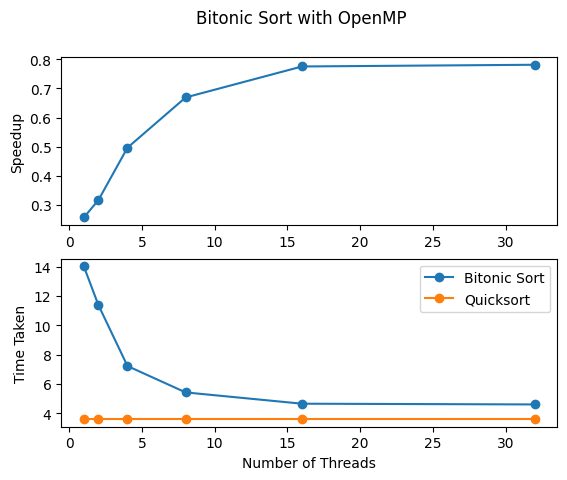
\includegraphics[width=0.5\textwidth]{pics/openmpres.png}
%     \caption{Results of the OPENMP implementation on different number of threads}
%     \label{fig:openmp_results}
% \end{figure}

\end{document}



